%%%%%%%%%%%%%%%%%%%%%%%% file template.tex %%%%%%%%%%%%%%%%%%%%%%%%%
%%
%% This is a general template file for the LaTeX package SVJour3
%% for Springer journals.          Springer Heidelberg 2006/03/15
%%
%% Copy it to a new file with a new name and use it as the basis
%% for your article. Delete % signs as needed.
%%
%% This template includes a few options for different layouts and
%% content for various journals. Please consult a p revious issue of
%% your journal as needed.
%%
%%
%% 5th Mar 2012
%% NOTES for MISTA 2015
%% This template has been supplied for use for the MISTA 2015 conference
%% In essence it is the same as the one supplied by SV, but with additional comments
%% The reason this template is being used is to make it as easy as possible
%% to be able to submit to the post conference special issue of the Journal
%% of Scheduling
%%%%%%%%%%%%%%%%%%%%%%%%%%%%%%%%%%%%%%%%%%%%%%%%%%%%%%%%%%%%%%%%%%%%
%%
%% First comes an example EPS file -- just ignore it and
%% proceed on the \documentclass line
%% your LaTeX will extract the file if required
%\begin{filecontents*}{example.eps}
%%!PS-Adobe-3.0 EPSF-3.0
%%%BoundingBox: 19 19 221 221
%%%CreationDate: Mon Sep 29 1997
%%%Creator: programmed by hand (JK)
%%%EndComments
%gsave
%newpath
%  20 20 moveto
%  20 220 lineto
%  220 220 lineto
%  220 20 lineto
%closepath
%2 setlinewidth
%gsave
%  .4 setgray fill
%grestore
%stroke
%grestore
%\end{filecontents*}
%%
%% For MISTA 2015, use the default option that has been supplied
%\documentclass{svjour3}                     % onecolumn (standard format)
%%\documentclass[smallextended]{svjour3}     % onecolumn (second format)
%%\documentclass[twocolumn]{svjour3}         % twocolumn
%%
%\smartqed  % flush right qed marks, e.g. at end of proof
%%
%\usepackage{graphicx}
%%
%% \usepackage{mathptmx}      % use Times fonts if available on your TeX system
%%
%% insert here the call for the packages your document requires
%\usepackage{latexsym}
%\usepackage{amsmath}
%\usepackage{amsfonts}
%\usepackage{graphicx}
%\usepackage{subfig}
%\usepackage{algorithmic}
%\usepackage{algorithm}
%\usepackage{enumerate}
%\usepackage{microtype}
%\usepackage{multirow}
%
%% please place your own definitions here and don't use \def but
%% \newcommand{}{}
%
%\newcommand{\xsc}{\gamma}
%\newcommand{\xSC}{\Gamma}
%
%\newcommand{\xs}{\boldsymbol{s}}
%\newcommand{\xd}{\boldsymbol{d}}
%\newcommand{\xq}{\boldsymbol{q}}
%\newcommand{\xb}{\boldsymbol{b}}
%\newcommand{\xl}{\boldsymbol{l}}
%\newcommand{\xf}{\boldsymbol{f}}
%\newcommand{\xD}{\boldsymbol{D}}
%\newcommand{\xt}{\boldsymbol{t}}
%\newcommand{\xe}{\epsilon}
%
%\newcommand{\xE}{\mathcal{E}}
%\newcommand{\xS}{\boldsymbol{S}}
%\newcommand{\xX}{\boldsymbol{X}}
%\newcommand{\xP}{\boldsymbol{\Pi}}
%\newtheorem{edit}{Edit}	
%\newtheorem{TODO}{TODO}
%
%% Insert the name of "your journal" with
%% This is preset for MISTA 2015: Do not change
%\journalname{MISTA 2015}
%%
%\setcounter{tocdepth}{3}
%\begin{document}
%
%\title{Exact and heuristic methods for trading-off makespan and stability in stochastic project scheduling} 
%\subtitle{}
%
%\author{Simon Mountakis \and
%	Tomas Klos \and \\
%	Cees Witteveen \and
%	Bob Huisman
%}
%
%\institute{Simon Mountakis \at
%	      Delft University of Technology \\
%	      \email{k.s.mountakis@tudelft.nl}  %  \\
%	   \and
%	   Tomas Klos \at
%	      Delft University of Technology \\
%	      \email{t.b.klos@tudelft.nl}  %  \\
%	   \and
%	   Cees Witteveen \at
%	      Delft University of Technology \\
%	      \email{c.witteveen@tudelft.nl}  %  \\
%	   \and
%	   Bob Huisman \at
%	      NedTrain \\
%	      \email{b.huisman@nedtrain.nl} %  \\
%}
%
%\maketitle
%
%\begin{abstract}
%This paper concerns networks of precedence constraints between tasks with random durations, 
known as stochastic task networks, often used to model uncertainty in real-world applications. 
In some applications, we must associate tasks with reliable start-times from which realized start-times will (most likely) not deviate too far.
We examine a dispatching strategy according to which a task starts as early as precedence constraints allow,
but not earlier than its corresponding \emph{planned release-time}.
As these release-times are spread farther apart on the time-axis, 
the randomness of realized start-times diminishes (i.e. \emph{stability} increases).
Effectively, task start-times becomes less sensitive to the outcome durations of their network predecessors.
With increasing stability, however, performance deteriorates (e.g. expected makespan increases).
Assuming a sample of the durations is given,
we define an LP for finding release-times that minimize the performance penalty of reaching a desired level of stability.
The resulting LP is costly to solve, so, targeting a specific part of the solution-space, 
we define an associated Simple Temporal Problem (STP) and show how optimal release-times can be constructed from its earliest-start-time solution.
Exploiting the special structure of this STP, we present our main result, 
a dynamic programming algorithm that finds optimal release-times with considerable efficiency gains.

%\end{abstract}
%
%%	\tableofcontents
%
\section{Introduction}
	
	% -- deterministic RCPSP
	
	Project scheduling literature mostly concentrates on scheduling
	subject to temporal and resource constraints.
	The schedule sought for is an assignment of start-times to activities,
	facilitating the efficient use of limited resources
	in order to minimize a lateness measure such as the project makespan.
	Finding a schedule usually invovles solving
	the Resource-Constrained Project Scheduling Problem (RCPSP) 
	(see \cite{artigues2013resource,hartmann2010survey} for comprehensive surveys).
	This problem has been shown to be \textsc{NP}-Hard \cite{blazewicz1983scheduling} and
	finds several industrial applications (e.g. \cite{bomsdorf2008model,bartels2009scheduling}).
	Associated literature includes numerous exact and (meta-)heuristic algorithms,
	able to find good schedules for large instances and diverse lateness measures
	(e.g. \cite{schutt2013solving,kone2011event,kolisch2006experimental,de2014novel}).
	%
	% -- transition from RCPSP to S-RCPSP because of uncertainty
	%
	Solving an RCPSP serves the purpose of preparing a feasible schedule,
	assuming a static deterministic project execution environment.
 	In practice, however, this assumption is rarely valid.
 	Activity durations used for preparing the schedule are mostly rough estimates,
 	since most projects are subject to delays during execution and
 	the final realized schedule is the result of 
 	subjecting the original schedule to modifications
 	which make it consistent with the project constraints in the face of delays.
 	Ad-hoc modifications lead to realized activity start-times 
 	that might differ from planned start-times,
  	compromising project predictability and timeliness.
	
	This paper addresses the issue of hedging against project uncertainty 
 	by preparing a schedule in combination with an execution strategy for coping with delays.
	In line with other works in \emph{stochastic project scheduling} 
	(see \cite{herroelen2004robust} for a comprehensive review)
	we assume activity durations are given as stochastic variables with known distributions
	and propose a new \emph{proactive-reactive} scheduling method.
	First, we define the Proactive Stochastic (PS) RCPSP as an extension of RCPSP.
	The solution to PS-RCPSP is a \emph{proactive schedule} and an \emph{earliest-start (es-) policy}
	that together minimize the weighted sum of the realized schedule's expected makespan 
	and its expected deviation from the proactive schedule.
	%
	PS-RCPSP is, in fact, a generalization of the Stochastic RCPSP (S-RCPSP),
	which asks to find a \emph{stochastic scheduling policy} instead of a schedule
	and various \emph{classes} of policies have been proposed in the literature 
	\cite{mohring1984stochastic,mohring1985stochastic,herroelen2004robust}.
	In general, a  policy defines a mapping between activity duration realizations to realized schedules.
	S-RCPSP asks to find a policy that minimizes the expected project makespan,
	with only few exact and heuristic approaches (mainly meta-heuristics) proposed over the last decade
	\cite{stork2000branch,ballestin2007worthwhile,ballestin2009resource,ashtiani2011new}.	
	
	Not preparing the project execution based on a schedule that can more or less be trusted
	(but rather, letting the realized schedule unfold during execution) 
	has been recognized as a shortcoming of S-RCPSP \cite{herroelen2004construction}.
	This shortcoming motivates us and a number of 
	other authors to propose a proactive-reactive approach,
	with \cite{van2008,deblaere2011proactive,lamas2015}
	yielding the most promising computational results in existing literature.
	Different approaches pursue different optimization objectives;
	however, the common aim is to optimize some \emph{tradeoff} between expected makespan 
	and expected deviation from the proactive schedule.
 	In line with other authors we represent activity duration distributions with a sample
 	and propose a Linear Programming (LP)-based heuristic for PS-RCPSP,
 	a Mixed-Integer LP (MILP) model enabling us to obtain exact solutions, and
 	a MILP-based heuristic which asimilates \emph{iterative flattening} \cite{oddi2009iterative}.
   	The (MI)LP models for PS-RCPSP proposed in this paper are the 
 	result of adjusting the models proposed by Artigues et al. in
 	\cite{artigues2003insertion} and \cite{leus2011robust}.	
 	We refer to exact solutions assuming stochastic duration distributions 
 	can be represented exactly by a sufficiently large sample.\footnote{
 	This notion of exactness is in line with Stork \cite{stork2000branch} who 
 	represent stochastic duration distributions with a sample
 	when proposing exact search methods for the S-RCPSP.}
 	
 	
%%%	Following the definition of PS-RCPSP we propose a heuristic based on Linear Programming (LP),
%%%	a Mixed Integer LP (MILP) model for PS-RCPSP that enables the finding exact solutions, and
%%%	a MILP-based heuristic that involves solving a sequence of smaller subproblems.
%%%	Similar proactive-reactive scheduling methods have been proposed by a number of authors,
%%%	with the heuristics in \cite{van2008,deblaere2011proactive,lamas2015} 
%%%	giving the most promising computational results.
%%%	Experiments with the known PSPLIB benchset \cite{kolisch1997psplib}
%%%	show that our heuristics compare favorably with prior art.
%%%	
%%%	This paper addresses the issue of hedging against project uncertainty 
%%% 	by preparing a schedule in combination with an execution strategy for coping with delays and
%%%	assuming activity durations are stochastic variables with known probability distributions.
%%% 	We propose a Mixed Integer Linear Programming (MILP) model along with two associated heuristics
%%% 	for a ploblem that we name the Proactive Stochastic RCPSP (PS-RCPSP).
%%% 	PS-RCPSP is, in fact, a generalization of an extension to the RCPSP,
%%% 	known as the Stochastic RCPSP (S-RCPSP),
%%% 	which is the main problem of study in the area of stochastic project scheduling \cite{herroelen2004robust}
%%%	(also known as reactive project scheduling).
%%%	S-RCPSP asks to find a \emph{stochastic scheduling policy} instead of a schedule.
%%%	Various \emph{classes} of policies have been proposed in the literature 
%%%	\cite{mohring1984stochastic,mohring1985stochastic,herroelen2004robust} but in general,
%%%	a policy is a combinatorial object representing a set of rules
%%%	that may guide the materialization of a final realized schedule,
%%%	as actual activity durations become known during project execution.
%%%	In effect, the policy defines a mapping from
%%%	every possible realization of activity durations to a corresponding realized schedule.
%%%	S-RCPSP asks to find a policy that minimizes the expected value of some project lateness measure
%%%	(e.g. the expected project makespan).
%%%	Few exact and heuristic S-RCPSP solution algorithms have been developed over the last decade
%%%	\cite{stork2000branch,ballestin2007worthwhile,ballestin2009resource,ashtiani2011new}.
%%%	
%%%	% -- transition from S-RCPSP to PS-RCPSP
%%%	
%%%	A main characteristic of S-RCPSP is that no schedule is prescribed prior to project execution.
%%%	Activity start-times are determined in a purely dynamic manner by the scheduling policy.
%%%	This has been recognized as a drawback (e.g. \cite{herroelen2004construction}) 
%%%	since the existence of a \emph{proactive}
%%%	schedule that can more or less be trusted may serve important organizational purposes.
%%%	An attempt to overcome this drawback gave rise to the research area of proactive-reactive project scheduling
%%%	which  is the research area that our work belongs to.
%%% 	The main idea behind the proactive-reactive approach is to execute the project by using
%%%	a proactive schedule together with a scheduling policy.
%%% 	The general aim of prominent approaches in this area 
%%%  	(e.g. \cite{van2008,deblaere2011proactive,lamas2015}) is to
%%% 	optimize some tradeoff between expected makespan and 
%%%	expected instability (deviation of the realized from the proactive schedule).
%%%		
%%%	The problem studied here, the PS-RCPSP, asks to find
%%%	a \emph{proactive} schedule paired with an \emph{earliest-start} (es) policy.
%%%	An es-policy is a set of temporal constraints between pairs of activities.
%%%	The proactive schedule prescribes release-times 
%%%	(i.e. earliest possible start-times) for activities.
%%%	An activity may start at its prescribed release-time or later in case of delays
%%%	(i.e. other activities requiring more than allocated time) as determined by the es-policy.
%%%	In effect, the tuple (proactive schedule, es-policy) defines a mapping from
%%%	every possible realization of activity durations to a corresponding realized schedule.
%%%	PS-RCPSP asks to find this tuple that minimizes 
%%%	the \emph{weighted sum} of two performance criteria:
%%%	\begin{enumerate}
%%%		\item expected project makespan,
%%%		\item expected tardiness with respect to the proactive schedule.
%%%	\end{enumerate}
%%%	The first criterion is relevant for obvious reasons.
%%%	The second criterion represents the extent to which the proactive start-times can be trusted.
%%% 	One typically wants to achieve low instability to avoid what is
%%% 	known as \emph{nervousness} \cite{steele1975nervous} and induces organizational costs.
 	
 	% -- paper structure and contributions
 	
	%This paper is about a problem of practical value in project scheduling:
	%trading expected makespan for stability under stochastic uncertainty.
	
	The contributions of this paper extend from section~\ref{sec-problem} and onwards.
	In order to base the paper on a consistent and self-contained framework of notation,
	section~\ref{sec-prelim} summarizes existing concepts from
	deterministic, reactive, and proactive-reactive project scheduling.
 	Section~\ref{sec-problem} introduces in a formal manner the problem studied here,
 	that we name Proactive Stochastic RCPSP.
	Section~\ref{sec-lp} presents one main contribution of this paper:
	a LP-based heuristic for solving this problem.
 	Section~\ref{sec-milp} presents another main contribution:
 	a MILP model for this problem which enables us to obtain exact PS-RCPSP solutions.
 	To our knowledge, no other exact solution methods have been proposed for poblems of similar type.
	Section~\ref{sec-milp-heuristic} presents yet another contribution,
	a MILP-based heuristic for PS-RCPSP.
	Section~\ref{sec-experiments} presents an experimental study in which we find
	that the LP-based heuristic performs favorably in comparison to the state-of-art,
	especially when the aim is to achieve near-zero instability.
	We also find the MILP-based heuristic to be more effective (albeit less efficient)
	when one is willing to accept medium levels of instability in order to minimize expected makespan.
	Section~\ref{sec-conclusion} concludes the paper.	
 	

\section{Preliminaries}
	\label{sec-prelim}
 	
 	The purpose of this section is to introduce the research area of
 	proactive-reactive (stochastic) project scheduling,
 	which is where the contributions of this paper belong to.
  	To establish autonomy and to facilitate discussion in further sections,
  	we use convenient notation (which sometimes departs from standard notation)
  	and begin with summarizing existing concepts from 
  	deterministic and (purely) reactive project scheduling.
  	For a comprehensive survey of deterministic,
  	reactive and proactive-reactive project scheduling,
  	the reader may refer to \cite{herroelen2004robust}.
   	 	
 	\subsection{Deterministic project scheduling}
 	 	
	A project is usually represented as a directed acyclic graph $G(N,E)$,
	with nodes $N=\{1,\ldots,n\}$ corresponding to the set of $n$ project activities.
	Each directed arc $(i,j)$ in $E \subseteq \{(i,j) \in N^2\}$ defines a direct
	temporal constraint between activities $i$ and $j$,
	meaning that $j$ may not start unless activity $i$ has finished.
 	In effect, $E$ defines a binary, irreflexive and transitive relation:
 	if there is a path from activity $i$ to activity 
 	$j$ in $G(N,E)$ then $j$ cannot start unless $i$ has finished.
	Let us $T(E) \supseteq E$ denote the transitive closure of $E$, 
	defined as 
	\[
		T(E) := \{(i,j) \in N^2 : \exists 
		\textrm{ a path from } i \textrm{ to } j \textrm { in } G(N,E)\}
	\]
	We shall name a \emph{temporally independent set} each
	subset of activities $X \subseteq N$ which are mutually 
	independent with respect to temporal constraints.
	That is, if $X$ is a temporally independent set, then $X^2 \cap T(E) = \emptyset$.
	Obviously, if only temporal constraints are taken into account, 
	the activities of a temporally independent set may overlap in time in a schedule.
	
	We assume as input a set $R := \{1,\ldots,m\}$ of $m$ resources which must be shared among activities.
	Each resource $r \in R$ is associated with known capacity $b_r \in \mathbb{N}_0$.
	Furthermore, each activity $i \in N$ requires a known amount 
	$q_{ir} \leq b_r$ of resource $r$ while it executes.
	Vector $\xb \in \mathbb{N}^m_0$ and matrix $\xq \in \mathbb{N}^{n \times m}_0$
	define the problem's resource constraints.
	Every independent set $X$ for which $\sum_{i\in X} q_{ir} > b_r$ 
	for some $r\in R$ is called a \emph{forbidden} set.
	Even though it is allowed by the temporal constraints $E$, 
	all activities in $X$ may not overlap at some timepoint $t$ because
	resource $r$ will be used beyond its capacity, which is not possible.
	
	Let $H \subseteq N^2$ denote a set of temporal constraints.
	Below we give the definition of a function $\Phi$ which returns the set of all forbidden sets
	w.r.t. temporal constraints $H$ and the problem's resource constraints $(\xq,\xb)$.
	\begin{align}
		\Phi(H) := \{X \subseteq N: 
		X^2 \cap T(H)=\emptyset, 
		\sum_{i\in X} q_{ir} > b_r \textrm{ for some } r \in R\}
	\end{align}
	
	In addition to the parameters mentioned so far,
	we assume as input a vector $\xd \in \mathbb{N}^n_0$ such that $d_i$ defines the duration of activity $i$.
	Overall, a tuple $(N,R,E,\xd,\xq,\xb)$ specifies an instance of the RCPSP.
	A schedule $\xs \in \mathbb{N}^n_0$ 
	such that $s_i$ defines the start time of activity $i$,
	is a feasible solution when it satisfies the temporal and resource constraints,
	meaning that
	\begin{align}
		s_j \geq s_i + d_i \qquad & \forall (i,j) \in E \label{eq-precon} \\
		a(\xs, t) \notin \Phi(E)	\label{eq-rescon} & \qquad \forall t \geq 0
	\end{align}
 
	Here, $a(\xs,t) := \{i \in N : t \in [s_i, s_i+d_i)\}$ is the set of
	activities executing at timepoint $t$ according to $\xs$ and $\Phi$ as defined earlier.
	Thus, (\ref{eq-rescon}) ensures there is no timepoint $t$ at which the
	activities of a forbidden set overlap concurrently.
	
	\paragraph{Project source-sink convention.}
	RCPSP asks to find a feasible schedule of minimum makespan
	$C_{\max}(\xs) := \max \{ s_i + d_i : i \in N\}$.
	Most RCPSP-related works assume that the last activity, $n$, 
	is a dummy activity with zero duration (i.e. $d_n = 0$) and that
	it must wait for the completion of every other activity (i.e. $(i,n) \in T(E)$ for every $i \in N-\{n\}$).
	This dummy activity is often known as the project "sink" and it holds that $C_{\max}(\xs) = s_n$.
	Another convention of most RCPSP-related works is that the first activity, 1,
	often known as the project "source" must be waited on by every other activity
	(i.e. $(1,j) \in T(E)$ for every $j \in N-\{1\}$).
	
 	We shall hereafter assume activities 1 and $n$ correspond to the project source and sink, respectively.
 	The RCPSP can now be formally stated as:
	\begin{align}
		\xs^* := \arg \min \{s_n:  (\ref{eq-precon}), (\ref{eq-rescon}), \xs \geq 0 \}
	\end{align}
	
	\subsection{Reactive project scheduling}
 	
	In the research area of stochastic project scheduling,
	the activity durations vector $\xd$ is replaced with a stochastic vector $\xD$ such that $D_i$
	is the stochastic variable representing the uncertain duration of activity $i$,
	with a known probability distribution $\mathbb{P}[D_i = t]$.
	In line with recent works on S-RCPSP,
	we shall denote (elements of) stochastic vectors with a capital symbol.
			
	S-RCPSP is a purely reactive extension of RCPSP.
	The solution sought for is no longer a schedule, but a reactive scheduling policy. 
	A policy is a combinatorial object $\pi$ which parameterizes the mapping  from stochatic vector $\xD$
	to a corresponding realized schedule $\xS(\pi,\xD)$.
	Note that $\xS$ denotes a function which returns a vector of activity start times (of length $n$).
	Furthermore, if a realization $\xd$ of $\xD$ is passed as an argument, 
	then $\xS(\pi,\xd)$ denotes a deterministic vector.
	if $\xD$ is passed as an argument, $\xS(\pi,\xD)$ denotes a stochatic vector.
	
	Different classes of policies have been proposed in the literature
	\cite{mohring1984stochastic,mohring1985stochastic,stork2000branch,ashtiani2011new}.
 	One condition that all policy classes are expected to satisfy is that function
 	$\xS$ complies with the \emph{non-anticipativity constraint}:
	the decision to start activity $i$ at time $[\xS(\pi,\xD)]_i$ cannot rely on information from the feature:
	the value of $[\xS(\pi,\xD)]_i$ must be determined by time $t \leq [\xS(\pi,\xD)]_i$.
	Other features such as the structure of $\pi$ and 
	the definition of function $\xS$ depend on the class under study.
	
 	\paragraph{List-based policies.}
	
	Two classes of policies which are prominent in the literature
	are \emph{resource-based} (rb) policies and \emph{activity-based} (ab) policies,
	also known collectively as \emph{list-based policies}.
	A list-based policy is a priority vector $\xl \in \mathbb{R}^n$ assigning priority $l_i$ to activity $i$.
	Realized schedule $\xS(\xl, \xD)$ is computed by a 
	variant of the well-known parallel schedule-generation-scheme (SGS)
	complying with the non-anticipativity constraint \cite{ballestin2009resource};
	with the SGS definition being slightly different between rb-policies and ab-policies.
%	At $t=0$ and at each subsequent activity completion $t > 0$
%	one starts as many activities as allowed by temporal and resource constraints.
%	A similar class is that of \emph{activity-based} (ab) policies;
%	an ab-policy is again a priority vector.
%	But the behavior of $p$ is now slightly different:
%	a activity may not start at $t$ 
%	(even if temporal and resource constraints allow this) unless 
%	all activities of lower priority have finished by $t$.
%	Note that every realized schedule $\xS(\xl,\xD)$ is feasible, 
% 	since function $\xS$ forces the problem's precedence and resource constraints
% 	regardless of the choice of $\xl$.
 	As far as list-based policies are concerned, S-RCPSP asks to find a vector 
	$\xl \in \mathbb{R}^n$ that minimizes $\mathbb{E}[[\xS(\xl,\xD)]_n]$.
	%
	Stork \cite{stork2000branch} proposes exact branch-and-bound algorithms for both rb and ab-policies.
	Ballest{\'\i}n \cite{ballestin2007worthwhile} proposes
	an efficient genetic algorithm for ab-policies,
 	providing the first computational experience on larger S-RCPSP instances.
	Ballest{\'\i}n and Leus \cite{ballestin2009resource} manage 
	to obtain better results with a 
	Greedy Randomized Adaptive Search Procedure (GRASP), 
	again for the class of ab-policies.
	The best performance (w.r.t. expected makespan minimization)
	has so far been obtained with the more recent work of
	Ashtiani et al. \cite{ashtiani2011new} who propose a GRASP
	for a new class, namely \emph{pre-processing} (pp) policies--%
	a hybrid between rb-policies and es-policies.

 	\paragraph{Earliest-start policies.}
 	
   	An es-policy is a set of temporal constraints $\xE \subseteq N^2$ chosen such that
 	\begin{align}
 		T(\xE) \supseteq E, \label{es-1} \\
 		\Phi(\xE) = \emptyset \label{es-2}, \\
 		G(N,\xE) \textrm{ is acyclic} \label{es-3}
 	\end{align}
 	Condition (\ref{es-1}) ensures that a schedule $\xs$ satisfying
 	$s_j \geq s_i + d_i$ for each $(i,j)\in \xE$ 
 	(here $\xd$ can be any arbitrary choice of activity durations)
 	is feasible with respect to the problem's precedence constraints $E$.
  	Condition (\ref{es-2}) ensures that
  	$\xs$ satisfying $\xE$ implies that it also satisfies resource constraints 
  	prescribed by availabilities $\xb$ and requirements $\xq$ (as described earlier).
 	Condition (\ref{es-3}) ensures that the set of schedules satisfying $\xE$ 
 	(for any arbitrary choice of activity durations $\xd$) is non-empty.
 	
 	When a project is executed according to an es-policy $\xE$,
 	the schedule that is realized, $\xS(\xE,\xD)$, 
 	is what is often known as the \emph{earliest-start} schedule specified by $\xE$.
 	The earliest-start schedule of $\xE$ can be defined as:
 	\begin{align}
 		[\xS(\xE,\xD)]_j := \max \{ [\xS(\xE,\xD)]_i + D_i : (i,j) \in \xE\}
 	\end{align}
 	To put it simply, an activity $j$ starts immediatelly 
 	when all its predecessors in $G(N,\xE)$ have finished.
  	This time quantity (the latest finish time of $j$'s predecessors)
  	is often known as the length of the \emph{critical path} from project source $1$ to activity $j$.
  	As far as es-policies are concerned, the S-RCPSP asks to find some $\xE^*$ which
  	minimizes $[\xS(\xE,\xD)]_n$ (the length of the critical path to the project sink) by expectation:
 	\begin{align}
 		\xE^* := \arg \min \{\mathbb{E}[[\xS(\xE,\xD)]_n] : (\ref{es-1} - \ref{es-3}), \xE \in N^2\}
 		\label{eq-s-rcpsp}
 	\end{align}
  	Constraints $(\ref{es-1} - \ref{es-3})$ enforce the feasibility of any realized schedule
  	with both the precedence and the resource constraints of the problem.
  	
	Stork \cite{stork2000branch} proposed an exact branch-and-bound search for problem (\ref{eq-s-rcpsp}).
	His algorithm considers each \emph{minimal} forbidden set $X$
	(subset-minimal forbidden set) in some order and branches
	on each of $|\{(i,j) \in X^2\}|$ arcs which can be included in $\xE$
	in order to eliminate $X$ from $\Phi(\xE)$.
	Without obtaining new computational results,
	in \cite{leus2011resource} Leus gives a formal treatment of
	es-policies as resource-flow networks
	(flow networks which can represent feasible RCPSP schedules) and
	proposes a refined version of the branch \& bound algorithm of Stork.
	Exploiting the relation between resource-flows and es-policies,
	Artigues et al. \cite{leus2011robust} propose a 
	robust optimization model for es-policies,
	for when a stochastic characterization of uncertainty is not available.
	
\subsection{Proactive-reactive project scheduling}
	
	Reactive project scheduling allows one to pick activity start times dynamically
	during the project, under conditions of uncertainty.
	A main drawback of this approach 
	(e.g. \cite{herroelen2004construction,herroelen2004robust,braeckmans2005proactive})
	is that prior to (and during) project execution there is no 
	schedule prescribing activity start times that can more or less be trusted.
	Such a "proactive" schedule can serve important organizational purposes;
	in fact, the deviation of the realized schedule from this proactive schedule
	is expected to induce organizational costs.
	
	Attempts to overcome this drawback gave rise to the research area of
	proactive-reactive project scheduling,
	which is the research area that this paper belongs to.
	The main idea behind the proactive-reactive approach is to execute the project by using
	a proactive schedule together with a scheduling policy.
	Under uncertainty, some activities may not start at their proactive start times,
	because activities they have to wait for are not yet finished and/or
	resources they require are not yet released.
	In such cases, the scheduling policy determines which activities to start at their
	prescribed start times and which to postpone.
	It should be noted that most works assume \emph{railway-mode scheduling},
	meaning that an activity may not start earlier than its proactive start time,
	which strengthens the "stability" of the project execution.
	Clearly, the realized schedule is a function of the policy and the proactive schedule.	
	Achieving low instability (deviation of the realized from the proactive schedule)
	requires "spreading" proactive activity start times far appart, 
	in effect increasing the expected makespan.
	The general aim is to optimize some tradeoff between expected makespan and expected instability.
	
	Van de Vonder et al. \cite{van2006trade,van2008,van2007heuristic} propose and
	evaluate experimentally various proactive-reactive heuristics.
	The proposed heuristics assume as input an instance of S-RCPSP along with an initial schedule.
	The best performing heuristic is the so-called Starting Time Criticality (STC) heuristic.
	An es-policy is extracted from the structure of this initial schedule and used to
	iteratively transform the initial schedule into a 
	proactive schedule by inserting time-buffers betwen activities.
	%
	Deblaere et al. \cite{deblaere2011proactive} propose 
	an approach which integrates the proactive step (forming a proactive schedule) 
	and the reactive step (forming the adjoining policy).
	Their approach is only possible to compare with ours and others that assume railway-mode scheduling,
	by choosing sufficiently high penalties for earliness (w.r.t. the proactive schedule).%
	\footnote{We are grateful to one of our anonymous reviewers for this remark.}
 	%
	More recently, Vilches and Demeulemeester  \cite{lamas2015}
	propose a Chance-Constrained Programming model (CCP) for the RCPSP
	which asks to find a minimum makespan schedule
	subject to probabilistic temporal and resource constraints.
	They propose a Mixed Integer LP model, 
	the solution to which is a proactive schedule that will most likely remain 
	feasible under stochastic duration variability,
	without presumption on the policy that will be used during project execution.

	\section{Proactive Stochastic RCPSP}
	\label{sec-problem}
		
	In deterministic and reactive project scheduling,
	the main problem under study (RCPSP and S-RCPSP, respectively) is stated clearly.
	A clearly stated problem model cannot be found in proactive-reactive project scheduling literature,
	perhaps because this research area is still in a burn-in phase.%
	\footnote{Some works refer to \cite{herroelen2004construction} but this is a formal treatment of a
	proactive-reactive \emph{machine} scheduling problem.}%
	Existing literature seems to pursue the general aim 
	of optimizing some tradeoff between expected makespan and 
	expected instability (deviation from the proactive schedule).
	This section presents the formal statement of a proactive-reactive scheduling problem for which
	(heuristic and exact) solution methods are proposed in subsequent sections.
	
	The problem presented here, the Proactive Stochastic RCPSP (PS-RCPSP), 
	asks to find a tuple $(\xE,\xt)$ where $\xE$ is an es-policy and $\xt$ is a proactive schedule,
	minimizing the weighted sum of two performance criteria:
	\begin{enumerate}
		\item expected value of project makespan,
		\item expected value of tardiness with respect to proactive release-times.
	\end{enumerate}
	The first criterion measures lack of robustness and is relevant for obvious reasons.
	The second criterion measures instability and captures the expected 
	deviation of the realized schedule from the proactive schedule.
	Note that $\xt$ prescribes activity release-times (an activity $i$ may not start earlier than $t_i$).
	Intuitively, instability represents the extent to which the proactive start-times can be trusted,
	when used for organizational purposes before and during project execution.
 	
 	An instance of this problem is encoded by a tuple $(n,m,\xq,\xb,E,\xD,\alpha)$.
 	For clarity, we summarize the meaning of problem parameters.
 	Positive integer $n$ is the number of activities and $m$ is the number of resources.
 	Parameters $\xq \in \mathbb{N}^{m\times n}_0$ and $\xb \in \mathbb{N}^m_0$ 
 	define resource requirements and availabilities respectively.
 	Set $E \subseteq \{1,\ldots,n\}^2$ defines pairwise precedence constraints.
 	Stochastic vector $\xD$ is of length $n$ with each element 
 	$D_i$ a stochatic variable (with given distribution $\mathbb{P}[D_i = t]$)
 	which describes the uncertain duration of activity $i$.
 	Finally, parameter $\alpha \in [0,1]$ determines the desired tradeoff between
 	robustness (i.e. minimization of expected makespan) 
 	and stability (i.e. minimization of expected instability).
  	More emphasis can be put on either minimizining makespan (by choosing $\alpha$ closer to one)
  	or minimizing instability (by choosing $\alpha$ closer to zero).
	
 	Formally, the problem can be stated as follows:
 	\begin{align}
 		\min \qquad & f(\xE, \xt) := \alpha \cdot \mathbb{E} \left[ [\xS((\xE,\xt),\xD)]_n \right] + 
 									(1-\alpha) \cdot \mathbb{E} \left[ \sum_{i=1}^n 
 									([\xS((\xE,\xt),\xD)]_i - t_i) \right] 
 									\label{eq-psrcpsp-obj} \\
 		\textrm{s.t.} \qquad	&	\Phi(G(N,\xE)) = \emptyset \label{eq-psrcpsp-1} \\
 								&	T(\xE) \supseteq E \label{eq-psrcpsp-2} \\
 								&	G(N,\xE) \textrm{ is acyclic} \label{eq-psrcpsp-3} \\
 								&	\xE \in \{1,\ldots,n\}^2, \xt \geq 0
 	\end{align}
 	Conditions (\ref{eq-psrcpsp-2},\ref{eq-psrcpsp-3}) ensure there is a non-empty
 	set of schedules satisfying the problem's precedence constraints as prescribed in $E$.
 	Condition (\ref{eq-psrcpsp-1}) ensures that each such schedule also satisfies the
 	problem's resource constraints prescribed by $\xq$ and $\xb$.
 
\section{Heuristic LP-based approach}
\label{sec-lp}
 	
 	This section presents a polynomial-time heuristic for PS-RCPSP which consists of two steps:
 	\begin{enumerate}
 		\item
 		using mean activity durations,
 		the deterministic RCPSP $(n,m,\xq,\xb,E,\mathbb{E}[\xD])$ is solved to obtain a good schedule $\xs$ and 
 		a feasible es-policy $\xE$ (i.e. satisfying (\ref{eq-psrcpsp-1}),(\ref{eq-psrcpsp-2}) and (\ref{eq-psrcpsp-3}))
 		is derived from the structure of $\xs$ in polynomial time 
 		(this procedure is described in \cite{artigues2003insertion}),
 		
 		\item
 		by solving a linear program presented below,
 		we find a proactive schedule $\xt$ that is optimally combined with $\xE$ (which is kept fixed)
 		so as to minimize an approximation of (\ref{eq-psrcpsp-obj}).
 	\end{enumerate}
  
 	After $\xE$ has been obtained in the first step,
 	finding $\xt$ which minimizes (an approximation of) the PS-RCPSP objective 
 	is achieved by solving the LP model presented below.	
 	
  	\begin{align}
 		\min \qquad & \left[ 
 			\alpha  \left( \frac{1}{|\xSC|} \sum_{\xsc \in \xSC} s^{\xsc}_n \right) +
 			(1-\alpha)  \left( \frac{1}{|\xSC|} \sum_{i=1}^{n}  \sum_{\xsc \in \xSC} (s^{\xsc}_i - t_i) \right)
  			\right] \label{eq-lp-obj} \\
 		\textrm{s.t.} \qquad & s^{\xsc}_j \geq s^{\xsc}_i + d^{\xsc}_i \qquad \forall (i,j) \in \xE, \xsc \in \xSC \\
 							 & s^{\xsc}_i \geq t_i \qquad \forall i=1,\ldots,n \\
 							 & \xt \geq 0
 	\end{align}
  	
 	Here, (\ref{eq-lp-obj}) approximates the objective (\ref{eq-psrcpsp-obj}) based on
 	$\Gamma \subseteq \mathbb{R}^n$:
    an adequately-sized sample of stochastic vector $\xD$.
  	The realization of activity durations under sample scenario $\xsc \in \Gamma$ 
 	is represented by vector $\xd^{\xsc} = (d^{\xsc}_1, \ldots, d^{\xsc}_n)$.
 	The corresponding realized schedule is 
 	$\textit{earliest-start}((\xE,\xt),\xd^{\xsc}) = (s^{\xsc}_1, \ldots, s^{\xsc}_n)$,
 	as computed by the model constraints.
 	The solution is a proactive schedule $\xt=(t_1,\ldots,t_n)$ that optimizes the tradeoff between
 	expected makespan and instability for the given es-policy $\xE$. 
 	This LP model has $n(|\Gamma|+1)$ linear variables 
 	($n$ variables $t_i$ and $n |\Gamma|$ variables $s^{\xsc}_i$).
 	

 \subsection{Related work}
\paragraph{Van de Vonder et al. \cite{van2008}} 

	propose several heuristics, 
  	of which the most competitive is the Starting Time Criticality (STC) 
 	heuristic and we shall therefore restrict our attention to it.
  	Our LP-based heuristic bears similarities with STC.
 	In fact, the first step of our heuristic is identical to that of STC:
 	an es-policy $\xE$ is extracted by the structure of an initial schedule $\xs$.
 	The second step of STC involves transforming the "unstable" schedule $\xs$
 	into a "stable" schedule $\xt$ with an iterative procedure, while keeping $\xE$ fixed.
 	In each iteration a one-unit time buffer is added at the start of that activity that "needs it the most" 
 	(as determined by a proposed "starting time criticality" measure)
 	until adding more buffer time would not further reduce the instability of $\xt$,
 	which is measured by
 	\begin{align}
 		\mathbb{E} \left[ \sum_{i=1}^n w_i ([\xS((\xE,\xt),\xD)]_i - t_i) \right] \label{eq-vonder-stb}
 	\end{align}
 	Here, $w_i$ is a cost associated with the instability of activity $i$.
 	Furthermore, $t_n$ is kept fixed to a project deadline and therefore $w_n$
 	represents the marginal cost of deviating from this project deadline.
 	Note that by replacing $\alpha$ in (\ref{eq-psrcpsp-obj}) 
 	with individual weights $w_i$ and choosing a fixed project deadline,
 	it is straightforward to adapt our approach to 
 	the instability objective considered by van de Vonder et al.
 	However, we felt that the choice of (\ref{eq-psrcpsp-obj}) as an objective is advantageous,
 	as it underlines the tradeoff between expected makespan and instability more clearly
 	and simplifies discussion by not involving a weight per individual activity and
 	not requiring the choice of a project deadline.
 	
	Note that $\xt$ is not guaranteed to be 
	(precedence and resource) feasible with respect to mean activity durations
	(as required in the work of van de Vonder \cite{van2008}).
	Enforcing $\xt$ to hold this property in our approach can be accomplished by
	including the following constraint in the LP model:
	\[
		t_j \geq t_i + \mathbb{E}[D_i] \qquad \forall (i,j) \in \xE
	\]
	However, this property only adds to the organizational value of $\xt$
	when mean values are reasonable estimates of activity durations.
	
	Let us note that both our heuristic and STC have 
	polynomial worst-case complexity (in the number of activities).
 	However, in contrast with STC, our approach guarantees that $\xt$ 
 	is chosen optimally when $\xE$ is kept fixed
 	and assuming the distribution of $\xD$ is approximated with a sample.
 	Therefore, if efficiency considerations enable us to choose a large-enough sample $\Gamma$
 	(which is mostly the case due to the efficiency of existing LP solvers),
 	our heuristic is expected to perform at least as well as STC.
 	Finally, note that our heuristic is simpler to implement,
 	requiring only the description of the presented LP model.

\paragraph{Leus et al. \cite{leus2004stability}}
assume as input a proactive schedule $\xt$ (e.g. one that has been produced by STC).
They propose a branch-and-bound search which returns the es-policy $\xE$ which fits $\xt$ optimally
in minimizing an expression of expected instability similar to (\ref{eq-vonder-stb}). 
\section{Exact MILP-based approach}
\label{sec-milp}
 	
 	PS-RCPSP (section~\ref{sec-problem}) asks to find an es-policy and a proactive schedule $(\xE,\xt)$
	that together minimize the weighted sum of expected makespan and instability.
	Section~\ref{sec-lp} presented a heuristic approach according to which 
	$\xE$ is kept fixed while $\xt$ is optimally paired with the policy by solving a LP.
	%
 	This section presents a Mixed Integer LP (MILP) model with which PS-RCPSP can be solved to optimality.
 	However, it should be pointed-out that a solution is trully exact only if we assume
 	stochastic duration distributions can be accurately described by the chosen sample $\Gamma$;
 	for general probability distributions we obtain a lower bound.
 	In fact, the problem of computing the exact expected makespan of a given es-policy
 	(and assuming duration distributions with discrete support) 
 	has been shown by Hagstrom in \cite{hagstrom1988computational} to be intractable.
 	However, our notion of exactness is in line with the computational study of Stork \cite{stork2000branch}
 	where "optimal" scheduling policies are computed by using a fixed sample of duration distributions.
 	
 	This model includes binary variables representing the 
 	structure of $\xE$ and linear variables representing $\xt$.
 	To our knowledge, no other exact approaches have been proposed in 
 	the literature for problems of similar type
 	(i.e. asking for a scheduling policy and proactive schedule that together optimize some
 	tradeoff between expected makespan and instability).
 	%In fact, and with the exception of \cite{deblaere2011proactive},
 	%existing heuristics for similar problems (e.g. \cite{van2008,lamas2015})
 	%do not attempt to optimize the scheduling policy and the proactive schedule together as a pair.
 	%
 	To arrive at this PS-RCPSP model, we merge the LP model presented in the previous section
 	with a MILP model that has been proposed by Artigues et al. \cite{artigues2003insertion}
 	and which allows to solve the deterministic RCPSP by treating it as a flow-network problem.
 	The model presented here is not entirely new,
 	since a similar technique (repeating precedence constraints for each
 	scenario of the chosen sample) has been proposed in \cite{leus2011robust}
 	for minimizing the maximum regret of an es-policy.
 		
	
\subsection{The RCPSP model of Artigues et al.}
	 
	Artigues et al. \cite{artigues2003insertion}
	represent a solution to the RCPSP as a so-called \emph{resource-flow}
	$\xf \in \mathbb{R}^{n\times n\times m}_0$;
	an assignment to variables $f_{ijr}$ associated 
	with each pair of activities $(i,j) \in N^2$ and each resource $r \in R$.
  	A resource-flow describes the "passing" of resource units inbetween activities.
 	More precisely, $\xf$ is an indirect representation of every schedule $\xs$ in which
 	$f_{ijr}$ units of resource $r$ are released by activity $i$ at its completion $s_i+d_i$
 	and then "picked up" by activity $j$ at its start $s_j$,
 	without another activity using these units between $s_i+d_i$ and $s_j$.
 	
 	A resource-flow is feasible when it satisfies
 	\begin{align}
 		\sum_{j \in N-\{i\}} f_{jir} = q_{ir}	\quad	\forall i \in N-\{1\} \label{eq-rf-1} \\
 		\sum_{j \in N-\{i\}} f_{ijr} = q_{ir} 	\quad	\forall i \in N-\{n\} \label{eq-rf-2}
  	\end{align}
 	Eq. $(\ref{eq-rf-1})$ asks that each activity $i$ (except for the sink)
 	receives as many resource units as it requires the moment it starts.
 	Eq. $(\ref{eq-rf-2})$ asks that each activity $i$ (except for the source)
	releases as many resource units as it has used the moment it finishes.
	
	The flow network $G(N,\phi(\xf))$ associated with $\xf$ is defined as
	$\phi(\xf) := \{(i,j) \in N^2: f_{ijr} > 0 \textrm{ for some } r \in R\}$;
	i.e. there is an arc from each activity to every other activity it
	passes at least one resource unit to.
  	As shown by Leus \cite{leus2011resource,leus2011robust},
  	feasible resource-flows and es-policies are interrelated:
  	$\xE = E \cup \phi(\xf)$ is a feasible es-policy if
  	$\xf$ is a feasible resource-flow (and $G(N,\xE)$ is acyclic).
  	Therefore, every schedule which satisfies $G(N,\xE)$ is feasible.
  	The following MILP model proposed by Artigues et al.
  	enables one to find a feasible resource-flow $\xf$
  	which minimizes the cost (described by function $g$)
  	of a schedule $\xs$ which satisfies the 
  	temporal constraints of $G(N,E \cup \phi(\xf))$.
  	
  	\begin{align}
  		\min \qquad			& s_n	\label{eq-art-obj}	\\
  		\textrm{s.t.} \qquad &	s_j \geq s_i + d_i - M(1-z_{ij}) \qquad \forall (i,j) \in N \label{eq-art-pre} \\
  			& z_{ij}=1 \qquad \forall (i,j) \in E \label{eq-art-zfix} \\
  			& f_{ijr} \leq M z_{ij} \qquad \forall (i,j) \in N^2, r\in R \label {eq-art-fz} \\
   			& (\ref{eq-rf-1}),(\ref{eq-rf-2}) \label{eq-art-inout} \\
  			& f_{ijr} \geq 0, z_{ij} \in \{0,1\} \qquad \forall (i,j) \in N^2, r\in R \label{eq-art-dom}
 	\end{align}
   	
%   	\begin{center}
%  	\begin{tabular}{ l l  r  l}
%  	min.	&	$s_n$									&	& \\
%  	s.t.	&	$f_{ijr} \leq M z_{ij}$					&	$\forall (i,j) \in N^2, r\in R$ & ($i$) \\
%  			&	$s_j \geq s_i + d_i - M(1-z_{ij})$		&	$\forall (i,j) \in N^2$	& ($ii$) \\
%  			&	$z_{ij} = 1$							&	$\forall (i,j) \in E$	& ($iii$) \\
%  			&	$f_{ijr} \geq 0, z_{ij} \in \{0,1\}$	&	$\forall (i,j) \in N^2, r\in R$ & ($iv$) \\
%  			&	(\ref{eq-rf-1}), (\ref{eq-rf-2})		& & ($v$)
%  	\end{tabular}
%  	\end{center}
  	
  	Here $M$ is a large constant.
  	Due to (\ref{eq-art-inout}) $\xf$ is a feasible resource-flow.
  	Due to (\ref{eq-art-fz}), if $f_{ijr} > 0$ for one or more $r \in R$ then $z_{ij} = 1$,
  	meaning that variables $z_{ij}$ describe the flow-network $\phi(\xf)$ of the resource-flow
  	(i.e. $\phi(\xf) = \{(i,j)\in N^2 : z_{ij}=1\}$).
  	Due to (\ref{eq-art-pre}) and (\ref{eq-art-zfix}), $\xs$ describes a schedule which 
  	satisfies the temporal constraints in $G(N,E\cup \phi(\xf))$.
  	Since $\xf$ is a feasible resource-flow, $\xs$ is a feasible schedule.
  	
\subsection{Extension for S-RCPSP}
  	
  	This section presents a trivial extension to the RCPSP model of Artigues et al.
  	which enables us to find optimal es-policies for the S-RCPSP.
   	Considering a sample $\Gamma \subset \mathbb{R}^n$ of stochastic activity durations vector $\xD$
   	allows us to present the following MILP model.
	
 	\begin{align}
 		\min \qquad 			& \frac{1}{|\xSC|} \sum_{\xsc \in \xSC} s^{\xsc}_n \label{eq-sart-obj} \\
 		\textrm{s.t.} \qquad	& s^{\xsc}_j \geq s^{\xsc}_i + d^{\xsc}_i - M(1-z_{ij}) 
 							   \qquad \forall (i,j) \in N^2, \xsc \in \xSC \label{eq-sart-pre} \\
 								& (\ref{eq-art-zfix} - \ref{eq-art-dom}) \label{eq-sart-dom}
 	\end{align}
   	
%  	\begin{center}
%  	\begin{tabular}{ l l  r  l}
%  	$\min$	&	$ \sum_{\gamma \in \Gamma}^n g(\xs^\gamma) $		&	& \\
%  	s.t.	&	$s^s_j \geq s^s_i + d^s_i - M(1-z_{ij})$	&	$\forall (i,j) \in N^2, s\in S$ & ($ii'$) \\
%  			&	(\ref{eq-rf-1}), (\ref{eq-rf-2}), ($i$), ($iii$), ($iv$)		& &	
%  	\end{tabular}
%  	\end{center}
  	
  	Our extension is rather straightfoward.
  	Each variable $s_i$ is included here as variable $s^{\xsc}_i$ for each sample scenario $\xsc \in \xSC$.
  	Precedence constraints (\ref{eq-art-pre}) from before are 
  	now replicated for each scenario $\xsc \in \xSC$ in condition (\ref{eq-sart-pre}).
  	Objective (\ref{eq-art-obj}) is now replaced with objective (\ref{eq-sart-obj}),
   	which estimates the makespan expectation $\mathbb{E}[S(E\cup \phi(\xf))]$ based on sample $\Gamma$.

\subsection{Extension for PS-RCPSP}
  	
  	Here we extend the previous model by including a variable $t_i$ for each $i\in N$,
  	which determines the activity's proactive starting time.
  	The resulting PS-RCPSP MILP model is presented below.
  	
  	\begin{align}
 		\min \qquad & \left [
 			\alpha  \left( \frac{1}{|\xSC|} \sum_{\xsc \in \xSC} s^{\xsc}_n \right) +
 			(1-\alpha)  \left( \frac{1}{|\xSC|} \sum_{i=1}^{n}  \sum_{\xsc \in \xSC} (s^{\xsc}_i - t_i) \right)
  			\right] \label{eq-milp-obj} \\
 		\textrm{s.t.} \qquad	& s^{\xsc}_j \geq s^{\xsc}_i + d^{\xsc}_i - M(1-z_{ij}) 
 							   \qquad \forall (i,j) \in N^2, \xsc \in \xSC \label{eq-milp-pre} \\
 								& (\ref{eq-art-zfix} - \ref{eq-art-dom}) \label{eq-milp-dom} \\
 								& s^{\xsc}_i \geq t_i \qquad i \in N \label{eq-milp-pro}, \xsc \in \xSC \\
 								& \xt \geq 0
 	\end{align} 	
 	
   	The objective now becomes identical to that of the LP-based heuristic,
  	measuring the weighted sum of expected makespan and expected instability.
  	Condition (\ref{eq-milp-pro}) ensures that an activity 
  	may not start earlier than its proactive start time.
  	
  	To summarize, by solving this model we obtain a PS-RCPSP solution $(\xE,\xt)$
  	where $\xE = \{(i,j) \in N^2: z_{ij} = 1\}$ is a feasible es-policy and $\xt$ defines a proactive schedule.
  	
 
 	\begin{proposition}
 	\label{pro-1}

 	Define $\xE := \{(i,j) : z_{ij} = 1\}$ the arcs of the flow-network
 	$G(N, E \cup \phi(\xf))$ associated with resource-flow $\xf$.
 	Let $\xf, \boldsymbol{z}, \xs, \xt$ be an optimal solution.
 	For each scenario $\xsc \in \xSC$,
 	$\xs^{\xsc}$ defines a schedule where each activity $i$ starts as soon as
 	allowed by its proactive release-time $t_i$ and es-policy $\xE$.
  	\end{proposition}
 	
 	\begin{proof}
 	For each scenario $\xsc \in \xSC$,
 	let $\bar{x}^{\xsc}$ denote the earliest allowed start time for activity $i$,
 	allowed by the combination of $\xE$ and proactive schedule $\xt$.
 	We want to prove that in an optimal solution, 
 	$\xs^{\xsc} = \bar{x}^{\xsc}$ for all $\xsc \in \xSC$.
 	
 	Assume that $s^{\xsc}_i = \bar{x}^{\xsc}_i + \delta$ for some $\xsc \in \xSC, i \in N$, with $\delta > 0$.
 	Since (\ref{eq-milp-obj}) increases monotonically with $s^{\xsc}_i$,
 	the objective can be improved by setting $s^{\xsc}_i = \bar{x}^{\xsc}_i$,
 	without violating any constraints.
 	Therefore, in every optimal solution we have $s^{\xsc}_i = \bar{x}^{\xsc}_i$ 
 	for all $\xsc \in \Gamma$ and $i \in N$,
 	meaning that each $\xs^{\xsc}$ defines the earliest start times schedule
 	allowed by the combination of by es-policy $\xE$ and proactive schedule $\xt$ under scenario $\xsc$.
 	\hfill $\Box$
 	\end{proof}
	
	By proposition~\ref{pro-1} it follows that an optimal solution to the MILP model
	presented above is, in fact, an optimal solution for the PS-RCPSP.


%\subsection{Related work}
%\paragraph{Braeckmans et al. \cite{braeckmans2005proactive}}
%\paragraph{Leus et al. \cite{leus2011robust}}
 
	\section{Heuristic MILP-based approach}
 	\label{sec-milp-heuristic}
  
 	
 	Even for small instances (e.g. with 30 activities and 4 resources),
 	solving the proposed model might take an inordinate amount of time.
 	We propose an algorithm (Algorithm~\ref{alg-milp-heuristic}),
 	the main idea of which was inspired by the \emph{iterative flattening}
 	heuristic of Oddi et al. \cite{oddi2009iterative}.
 	The heuristic of Oddi et al. was developed for the
 	deterministic RCPSP with minimum/maximum time-lag precedence constraints \cite{herroelen2001note}.
 	Every feasible schedule for the problem they study is compactly represented 
 	as a network of temporal constraints (known as a Simple Temporal Network \cite{dechter1991}).
 	It is the similarity with an es-policy (which is a network of zero-lag temporal constraints)
 	that has inspired the development of the heuristic presented here. 
  
 	The proposed heuristic involves solving a sequence of 
 	sufficiently small subproblems with non-increasing optimal objective values.
 	Each iteration involves solving a partially solved instance to optimality.
 	Thus, worst-case complexity is exponential in the number of activities.
 	In practice, however, "good" solutions can be obtained with relative efficiency.
  	
 	\begin{algorithm}
 		\caption{Iterative flattening for PS-RCPSP}
 		\label{alg-milp-heuristic}
 		\begin{algorithmic}[1]
 		\State $\xs \leftarrow$ schedule for RCPSP $(N,R,E,\mathbb{E}[\xD],\xq,\xb)$
 		\State $\xE^{*} \leftarrow E \cup \phi(\xf^{\xs})$ with $\xf^{\xs}$ extracted from $\xs$
 		\State $\xt^{*} \leftarrow (0,\ldots,0)$
 		%\State $k \leftarrow 0$
 		
 		\While {termination criteria not met}
 			\State $\mathcal{H} \leftarrow$ random subset of $\xE^{*}-T(E)$ chosen by criticality probability
 			\State $(\xE,\xt) \leftarrow$ 
 					optimal solution for PS-RCPSP $(N,R,\xE^{*}-\mathcal{H},\xD,\xq,\xb,\alpha)$
 			\If {$(\xE,\xt)$ has a lower objective than $(\xE^{*},\xt^{*})$}
 				\State $(\xE^{*},\xt^{*}) \leftarrow (\xE,\xt)$
  			\EndIf
  			%\State $k \leftarrow k + 1$
 		\EndWhile
 		\State return $(\xE^{*},\xt^{*})$
 		\end{algorithmic}
 	\end{algorithm}	
 	
 	Algorithm~\ref{alg-milp-heuristic} assumes as input an instance of the
 	PS-RCPSP.
 	According to aforementioned notation,
 	the instance is represented as $(N,R,E,\xD,\xq,\xb,\alpha)$.
 	An initial solution is obtained by solving a
 	deterministic RCPSP (lines 1-3)
 	which can be done efficiently with one of the various existing heuristics.
 	This solution will serve as a starting point for the first iteration,
 	which is described as follows.
 	A partial solution is formed by removing a random 
 	subset of highly critical arcs from the current solution (line 6).
 	The resulting subproblem is solved to optimality (by use of the proposed model)
 	and a complete solution is obtained (line 7).
 	If this new solution is better,
 	it becomes the starting point of the next iteration.
 	The algorithm may terminate when, e.g., a chosen
 	number of iterations have been performed,
 	or the objective has failed to improve a certain number of times. 
 	
 	\paragraph{Further efficiency improvements.}
 	Note that the optimal solution $(\xE,\xt)$   
 	of the subproblem solved in each iteration
 	cannot be worse than the best solution seen so far, $(\xE^*,\xt^*)$.
 	To improve performance one may use $(\xE^*,\xt^*)$ as an initial solution when solving the model (line 6).
 	Efficiency can be further improved by reducing the number of binary variables $z_{ij}$ in the model.
 	This can be accomplished by observing that
 	$z_{ij}$ for each $(i,j) \in T(\xE^* -  \mathcal{H})$ can be fixed to one and
 	$z_{ij}$ for each $(j,i) \in  T(\xE^* - \mathcal{H})$ can be fixed to zero.
 
\section{Experiments} 
\label{sec-experiments}	
 
 	In \cite{lamas2015}, Vilches and Demeulemeester 
 	compare their method (CCP) with 
 	that by Van de Vonder et al. (STC) \cite{van2008}.
 	To the best of our knowledge, STC and CCP constitute the state-of-art as far as
 	trading expected makespan for instability in stochastic project scheduling is concerned.
 	In this section we extend this comparison by using the same experimental set-up
 	and including results for our LP-based heuristic (Section~\ref{sec-lp}) and 
 	the MILP-based heuristic (Section~\ref{sec-milp-heuristic}).
 	As the results show, our approaches compare favorably with STC and CCP.  

  	The set-up used in \cite{lamas2015} was based 
  	on the \texttt{J30} deterministic RCPSP bench-set of the well-known PSPLIB \cite{kolisch1997psplib},
 	which comprises 480 deterministic RCPSP instances, each with $n=30$ activities.
 	Based on this bench-set, three stochastic RCPSP bench-sets were derived, 
 	namely \texttt{J30-low}, \texttt{J30-med}, and \texttt{J30-high},
  	corresponding to conditions of low, medium, and high project uncertainty,
 	with activity durations following a discretized beta distribution.
 	Specifically, each activity $i$ with duration $d_i$ in the deterministic RCPCP instance
 	now has stochastic duration $D_i = [X_i d_i 0.5 (l + h)]$ with $\mathbb{E}[D_i] \simeq d_i$ where
 	\begin{itemize}
 		\item $X_i$ follows a beta distribution with shape parameters $\alpha=2, \beta=5$;
 		\item $l = 0.75$ and $h = 1.625$ in the low variability bench-set;
 		\item $l = 0.5$ and $h = 2.25$ in the medium variability bench-set;
 		\item $l = 0.25$ and $h = 2.875$ in the high variability bench-set;
 		\item operator $[\cdot]$ represents rounding to the closest integer.
 	\end{itemize}

 	Each of the evaluated methods (including STC and CCP) has a certain "tradeoff parameter"
 	which determines whether more emphasis is put on minimizing
 	expected makespan or minimizing expected instability.
 	For our LP-based and MILP-based heuristic this tradeoff parameter 
 	is the weight $\alpha$ in expression (\ref{eq-psrcpsp-obj}).  
 	CCP and STC have corresponding parameters with a similar effect.
 	By varying the choice of the corresponding tradeoff parameter(s),
 	a set of tradeoff data-points is obtained for each method, on each of the three bench-sets.
  
 	\begin{figure} 
 		\centering   
   		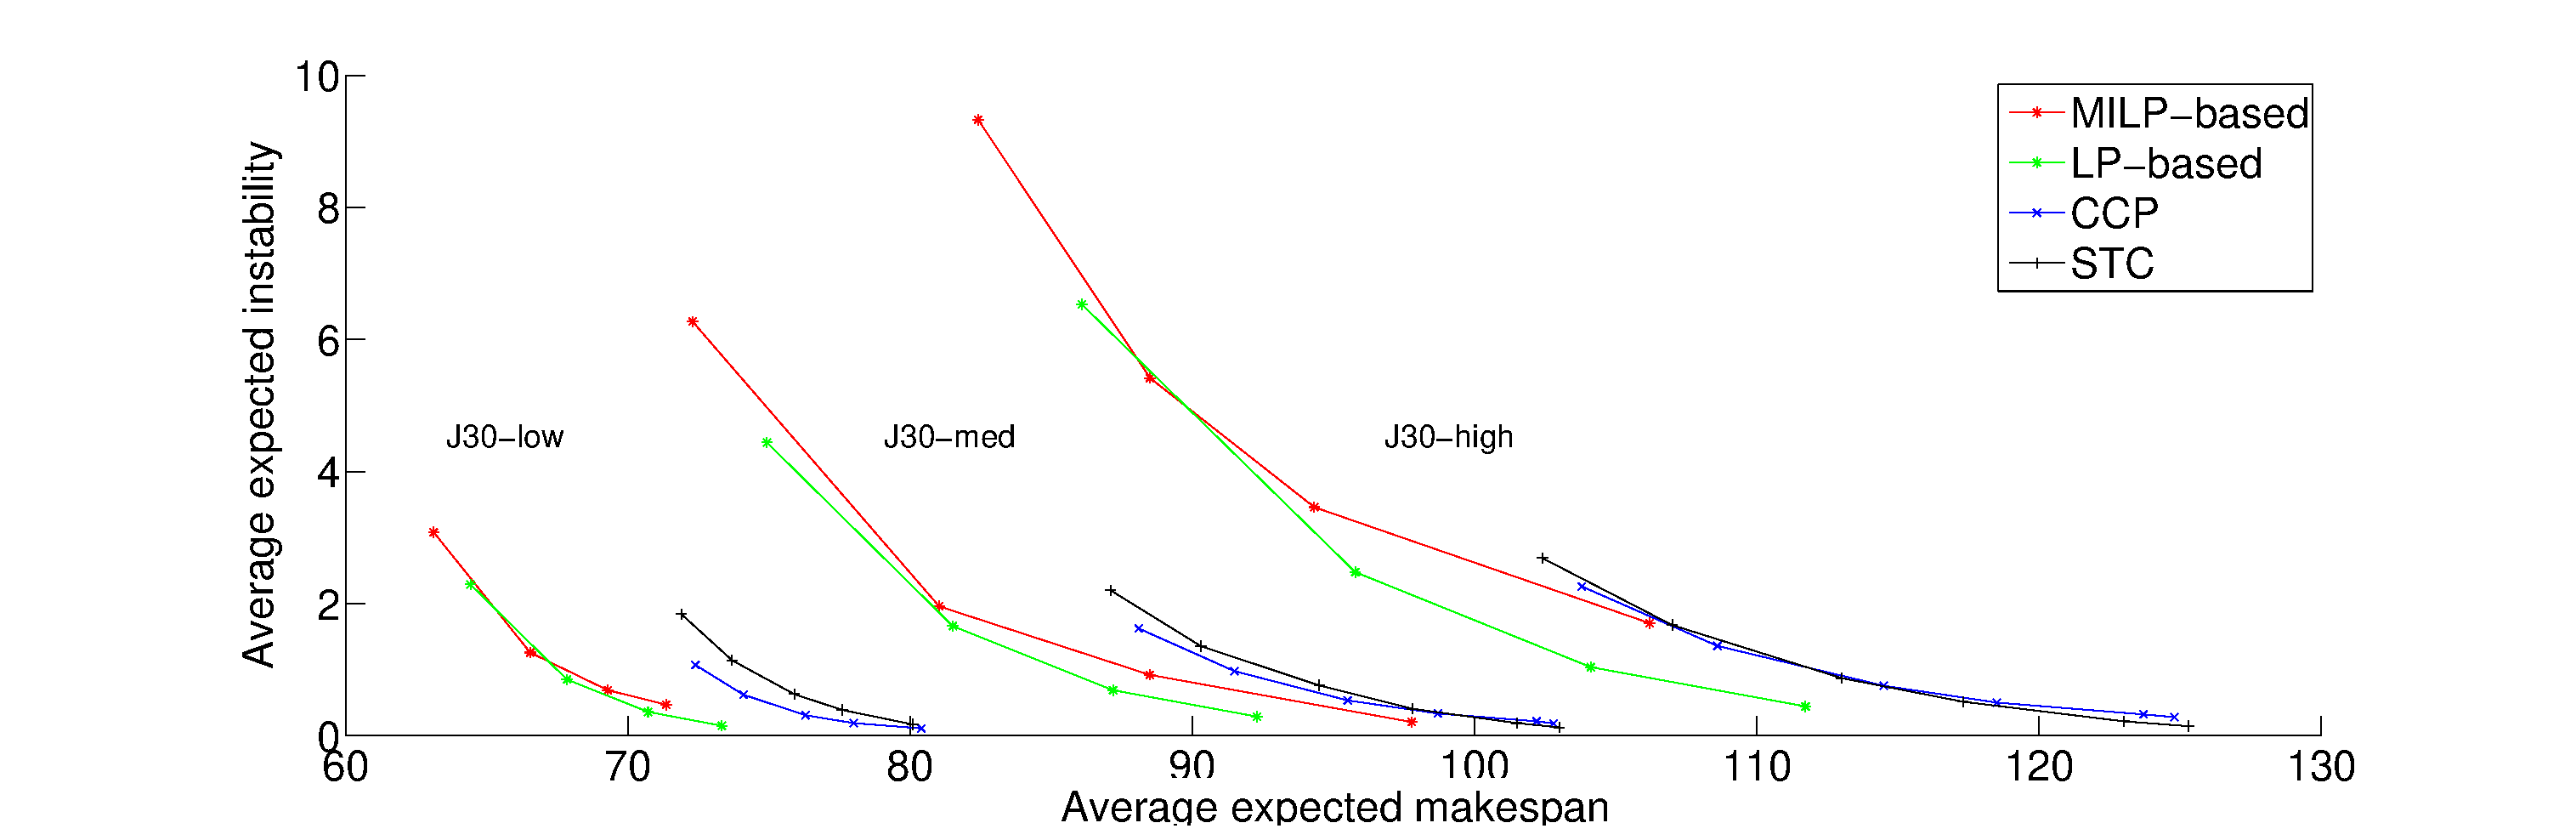
\includegraphics[width=1.0\textwidth]{chapter/mista-stability/figure1.eps}
 		\caption{Trading expected makespan for stability.}
 		\label{fig-experiments-1}
 	\end{figure}
 	
  	\begin{figure} 
 		\centering  
   		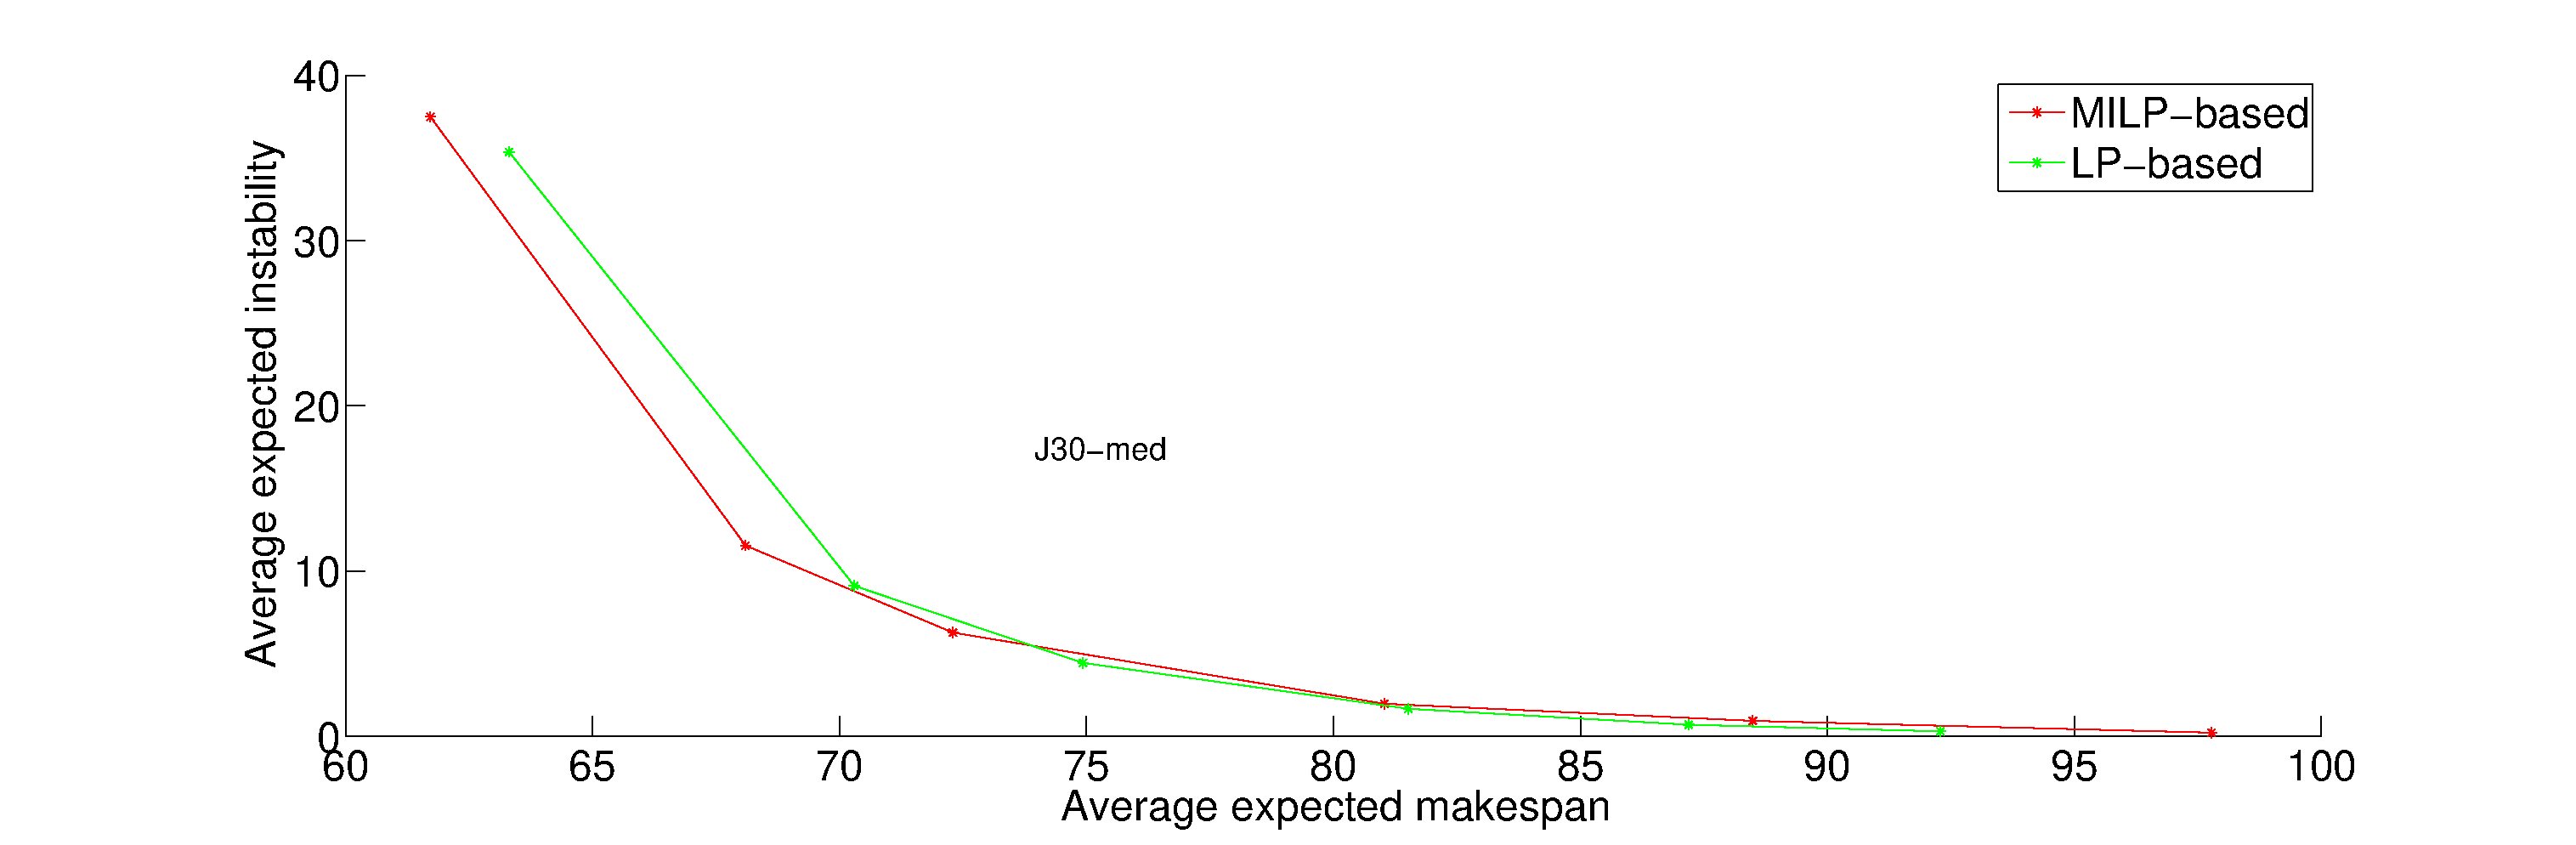
\includegraphics[width=1.0\textwidth]{chapter/mista-stability/figure2.eps}
 		\caption{Trading expected makespan for stability for higher $\alpha$.}
 		\label{fig-experiments-2}
 	\end{figure}
 	
 	In Figure~\ref{fig-experiments-1},
 	the data-points for each method are displayed as a tradeoff curve, 
 	on each of the three bench-sets, resulting in three "clusters" of tradeoff curves.
 	A tradeoff curve captures the average performance of the method on that bench-set.
 	Specifically, each data-point is two-dimensional and records the average expected makespan and average 
 	expected instability for a certain choice of the tradeoff parameter(s),
 	where the average is taken over all 480 instances of the bench-set.
  	Data-points for CCP and STC are borrowed
 	from the work of Vilches and Demeulemeester \cite{lamas2015}.	
  	Data-points for our heuristics are obtained by setting $\alpha=0.05$, $0.1$, $0.2$, and $0.4$.
 	Higher alpha values correspond to data-points closer to the upper left corner,
 	with higher instability and lower makespan.	
 	
 	Figure~\ref{fig-experiments-2} focuses on the medium variability case for higher $\alpha$ values,
 	including additional data-points for $\alpha=0.6$ and $\alpha=0.9$.
 	This allows us to compare the MILP-based and LP-based heuristics when
 	more emphasis is put on minimizing expected makespan.
 	
 	The expected makespan and expected instability of the solution
 	provided by each of the methods on a particular instance
 	is computed with a sample $\Gamma^{large} \subset \mathbb{R}^n$ 
 	comprising $|\Gamma^{large}| = 10^3$ realization of durations vector $\xD$.
 	Note that the data-points of Vilches and Demeulemeester were computed with a different sample of size $10^3$.
 	We assume that $10^3$ is a sufficiently large sample size to facilitate comparability with our results.
 	
 	\paragraph{Configuration of heuristics.}
 	The sample $\Gamma^{milp}$ used by our MILP-based heuristic during optimization
 	(see line 6 of Algorithm~\ref{alg-milp-heuristic}) is of size $|\Gamma^{milp}| = 30$.
 	Our MILP-based heuristic is configured to perform three (3) iterations and
 	the number of highly critical arcs removed in each iteration 
 	(see line 5 of Algorithm~\ref{alg-milp-heuristic}) is $|\mathcal{H}| = 20$.
 	Note that the criticality of the arcs is computed based on sample $\Gamma^{large}$
 	(this is done efficiently, in time quadratic in $n$ and linear in $|\Gamma^{large}|$).
  	The solver we use is \textsc{CPLEX} version 12.6.
  	Furthermore, we set a time-limit for the solver to 50 seconds
  	(since each iteration starts from a feasible solution, 
  	the solver will always return with a solution within the time-limit).
  	The polynomial-time complexity of our LP-based heuristic (no binary variables in the model)
  	allows us to use a large sample during optimization.
  	In fact, we use sample $\Gamma^{large}$.
  	To find a deterministic schedule (as required in step 1 of this LP-based heuristic)
  	we used a priority rule procedure recently proposed in \cite{de2014novel}.
  	Vilches and Demeulemeester use a sample of size $10^2$ during optimization, for both STC and CCP.
  	Furthermore, they limit the time spent in solving their 
  	CCP model on an instance to a maximum of 10 seconds. 
 
   	
  	\paragraph{Observations.}
  	Figure~\ref{fig-experiments-1} suggests that
   	regardless of the mode of variability (low, medium, or high),
  	when the purpose is to achieve near-zero instability,
  	the LP-based heuristic yields the best results.
  	This can be attributed to the efficiency of solving a LP model,
  	which enables us to use a large sample (of size $10^3$ in this case) during optimization.
  	
  	Figure~\ref{fig-experiments-2} suggests that
  	even though the sample used during optimization is much smaller
  	for the MILP-based heuristic (of size $30$),
  	it is more effective than the LP-based heuristic for higher $\alpha$ values
  	(i.e. when minimizing instability is  more important than minimizing makespan).
  	Both the LP-based and the MILP-based heuristics start from the same es-policy
  	(see step 1 in section~\ref{sec-lp} and line 2 of Algorithm~\ref{alg-milp-heuristic}, respectively).
  	However, the MILP-based heuristic restructures the policy and this enables
  	it to perform better at minimizing expected makespan.
  	
  	Restructuring the policy comes at the cost of efficiency.
   	With three iterations allowed per instance,
  	this yields an average of 50 seconds per instance for the MILP-based heuristic.
  	The LP-based heuristic is considerably more efficient, with an average of 1.5 seconds per instance.
  	Vilches and Demeulemeester report that STC spends on average 0.2 seconds per instance,
  	while their CCP approach spends on average 10 seconds per instance. 
 	

\section{Conclusions and future work}
\label{sec-conclusion}

This paper proposes the PS-RCPSP problem model which,
assuming stochastic activity durations,
asks to find a so-called earliest-start (es) policy and
a proactive schedule that together minimize the weighted 
sum of expected project makespan and expected instability.
Extending an existing MILP model for the RCPSP,
a MILP model for PS-RCPSP is presented, which allows us to 
find optimal (es-policy, proactive schedule) pairs.
Solving this problem to optimality might require an impractical amount of time,
even for instances with few activities (e.g. 30).
Therefore, we propose a LP-based and a MILP-based heuristic for the PS-RCPSP.
Our LP-based heuristic optimizes the proactive schedule by keeping the es-policy part of the  solution fixed.
Our MILP-based heuristic optimizes the structure of the policy together with the proactive schedule.
The LP-based heuristic, which is rather efficient, seems to be more effective compared to the state-of-art
(i.e. achieves smaller expected makespan for a certain level of expected instability) especially
when the aim is to achieve close to zero instability.
The MILP-based heuristic is rather effective when the aim is to
achieve low expected makespan at the cost of moderate or high instability.
In contrast to existing state-of-art approaches such as
CCP \cite{lamas2015} and STC \cite{van2008},
our heuristics rely on the idea of optimizing 
the proactive schedule together with the scheduling policy.
This difference might in part explain observed performance differences.

Future work involves a thorough experimental analysis of the proposed heuristics,
not for the purpose of comparing them to the state-of-art,
but for a deeper understanding of their behavior and its
dependence on problem characteristics.
Furthermore, most existing stochastic project scheduling works are evaluated on instances where
the deterministic RCPSP counterpart instance 
(formed by mean activity durations) serves as a good approximation of the stochastic instance.
This is exploited by our heuristics and other heuristics such as STC.
However, in certain practical domains (e.g. maintenance scheduling),
the duration of some activities is known a-priori with accuracy,
while the duration of other activities follows a distribution with very high variance.
In maintenance scheduling, for example, "inspection" activities have known durations
but "repair" activities might be (un)necessary with certain probabilities. 
We would like to investigate performance on such instances 
which cannot be approximated well by their determinitic counterpart.
%
%\begin{acknowledgements}
%We would like to thank our anonymous reviewers for their constructive remarks.
%This research belongs to the \emph{Job Scheduling Problem} part of the 
%\emph{Rolling Stock Life Cycle Logistics} applied research and development programme, 
%funded by \emph{NS/NedTrain}.
%\end{acknowledgements}
%
%% BibTeX users please use one of
%\bibliographystyle{plain}      % basic style, author-year citations
%%\bibliographystyle{spmpsci}      % mathematics and physical sciences
%%\bibliographystyle{spphys}       % APS-like style for physics
%\bibliography{p}   % name your BibTeX data base
%
%% Non-BibTeX users please use
%%\begin{thebibliography}{}
%%
%% and use \bibitem to create references. Consult the Instructions
%% for authors for reference list style.
%%
%%\bibitem{RefJ}
%% Format for Journal Reference
%%Author, Article title, Journal, Volume, page numbers (year)
%% Format for books
%%\bibitem{RefB}
%%Author, Book title, page numbers. Publisher, place (year)
%% etc
%%\end{thebibliography}
%
%\end{document}
%% end of file sample.tex
%
%
